\section{Αρχιτεκτονική προγραμματιστικού περιβάλλοντος}
\begin{frame}
	\frametitle{Αρχιτεκτονική προγραμματιστικού περιβάλλοντος}

	\centering
	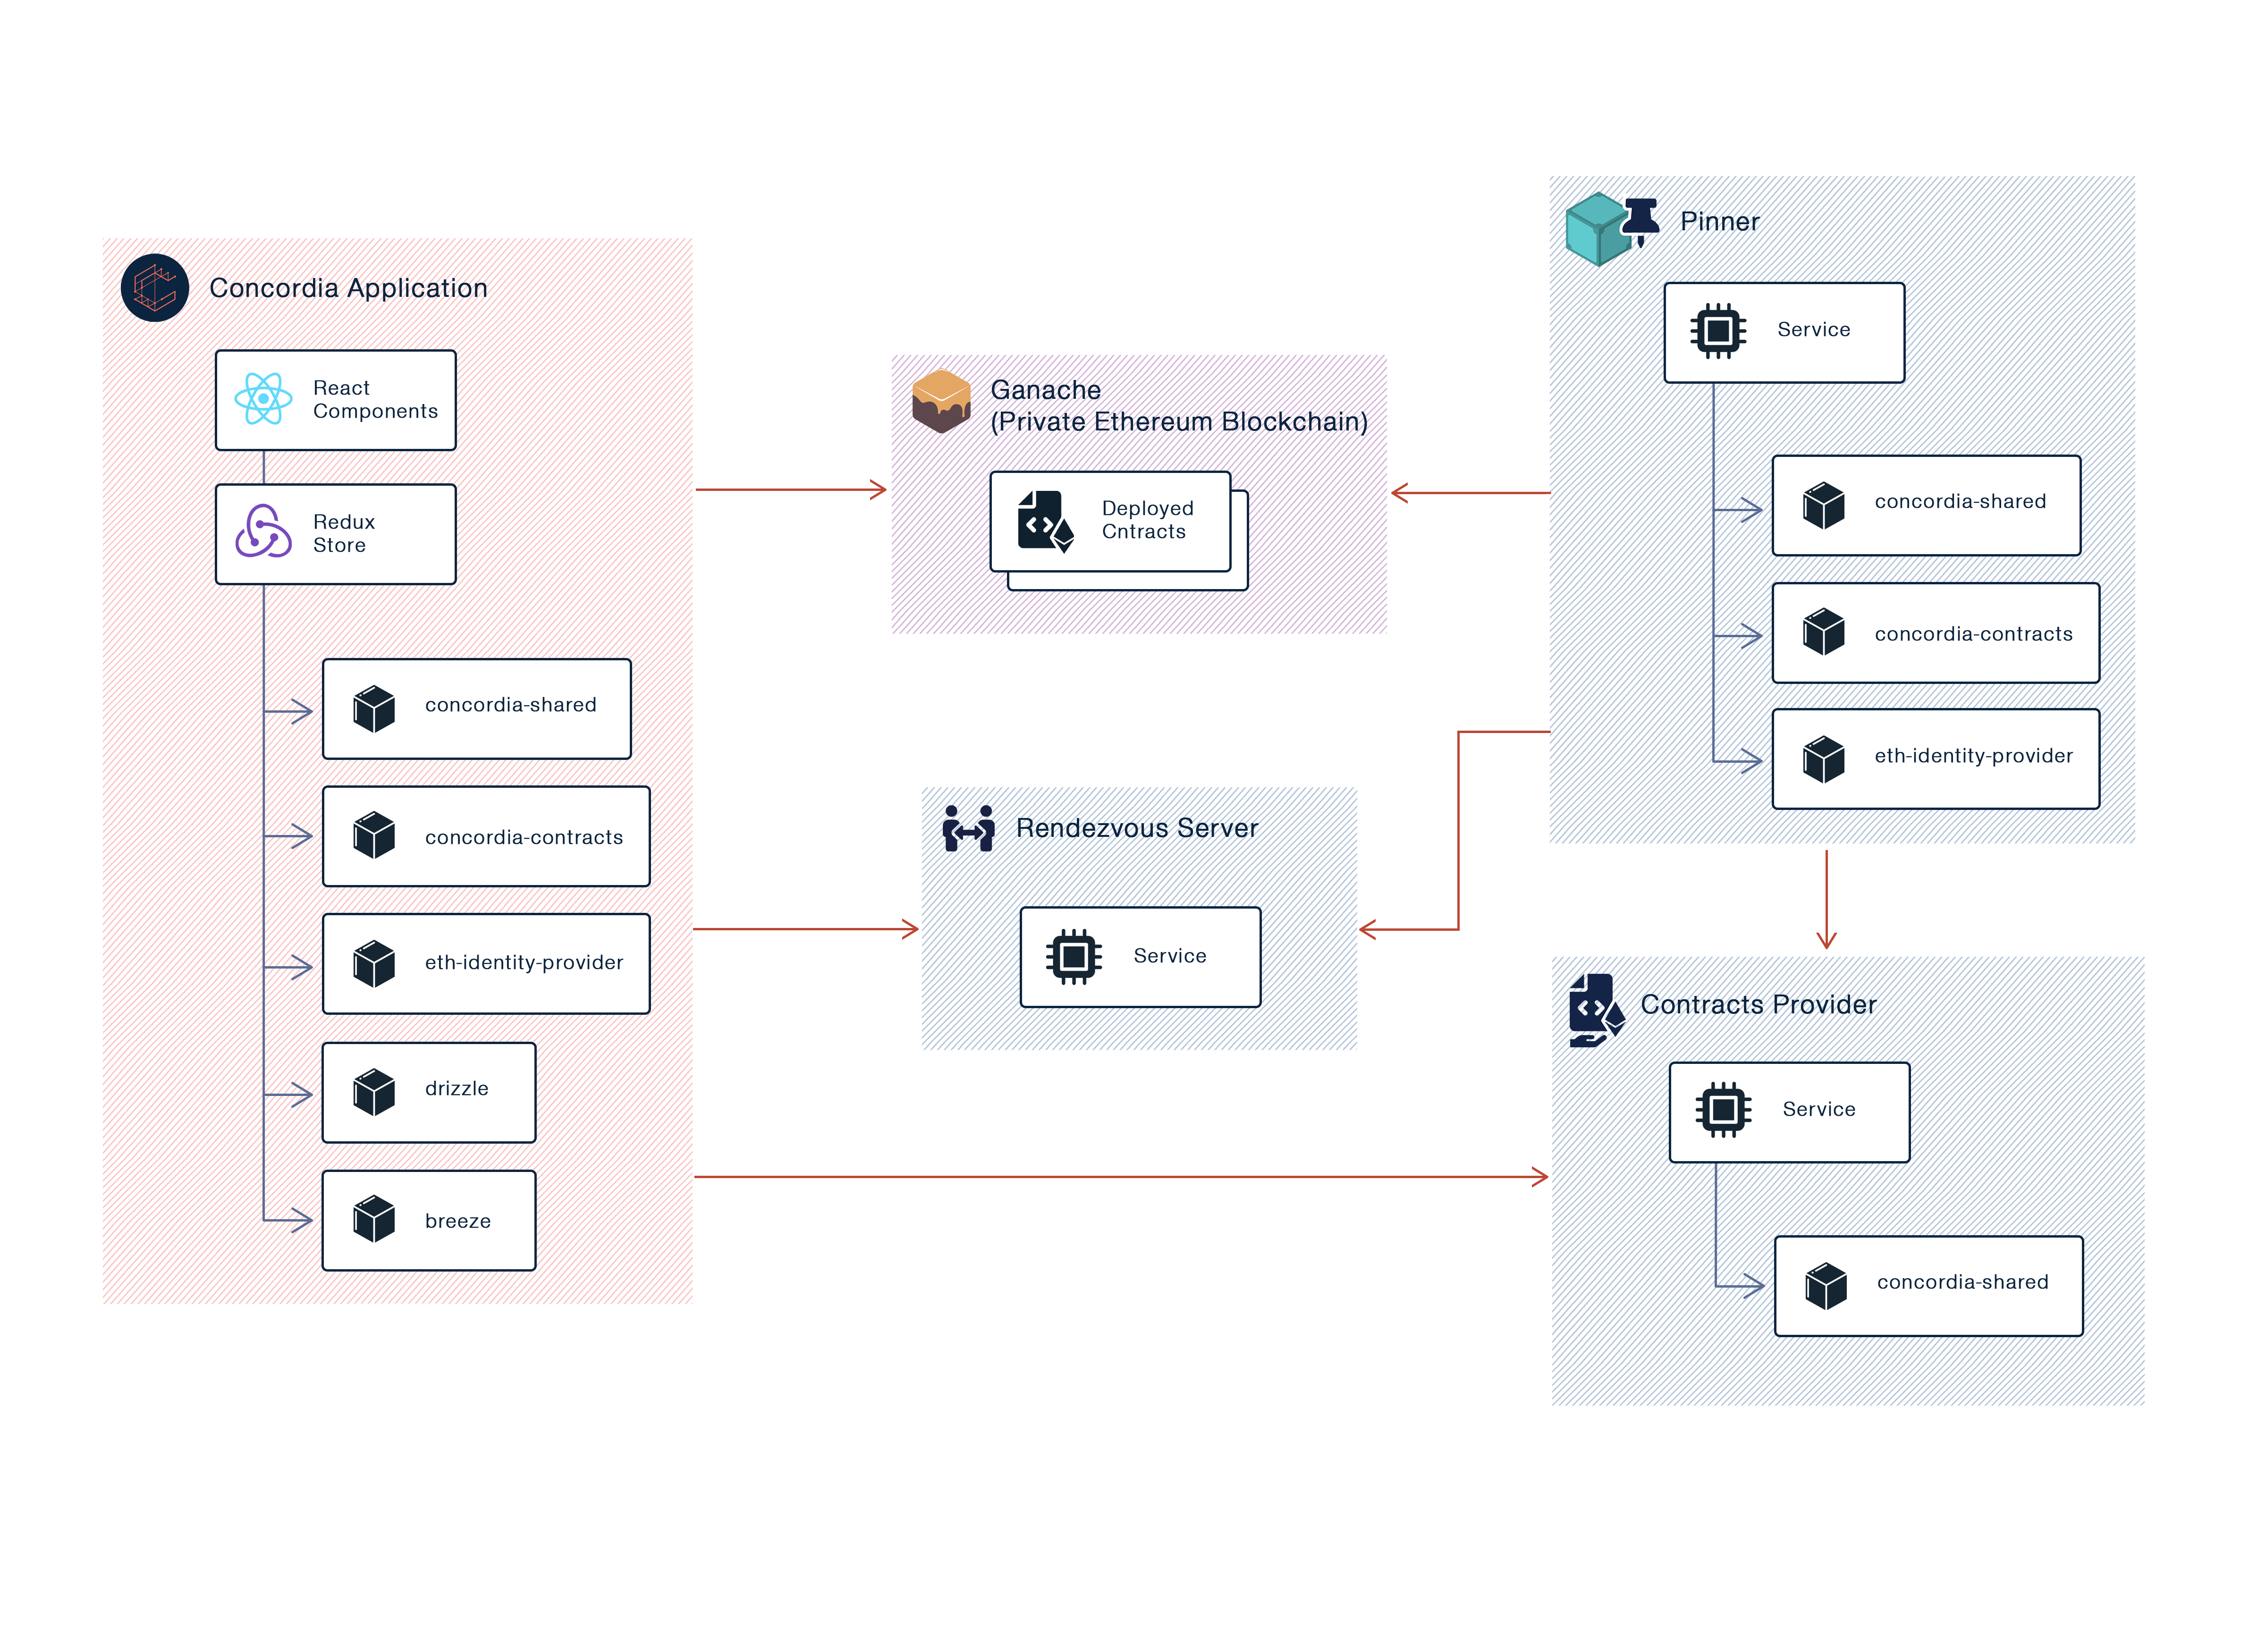
\includegraphics[width=\textwidth]{assets/figures/architecture-overview.png}
\end{frame}

\note{
	Εδώ θα δούμε τον τρόπο με τον οποίο χρησιμοποιήθηκαν οι τεχνολογίες που αναφέραμε προηγουμένως, την σχεδίαση της πλατφόρμας σε υψηλό επίπεδο καθώς και την αλληλεπίδραση των επιμέρους συστημάτων.

	Το βασικότερο μέρος της πλατφόρμας είναι η εφαρμογή (Concordia Application). Αυτό αποτελεί μία διαδικτυακή εφαρμογή με μορφή ιστοσελίδας. Εκθέτει τις γραφικές διεπαφές μέσω των οποίων αλληλεπιδρούν οι χρήστες με την πλατφόρμα. Στην εφαρμογή αυτή χρησιμοποιούνται αρθρώματα (διακριτά μέρη κώδικα) που διαχειρίζονται τις απαραίτητες διαδικασίες, όπως οι συναλλαγές με το blockchain και η αποθήκευση στο IPFS.

	Ο rendezvous server είναι ένα λογισμικό απαραίτητο για την χρήση του IPFS. Διατηρεί μία λίστα των διευθύνσεων των χρηστών που είναι ενεργοί στο σύστημα κάθε στιγμή, την οποία παρέχει σε νέους χρήστες που εισέρχονται σε αυτό. Έτσι, μέσω του server αυτού γίνεται η ανακάλυψη ομότιμων κόμβων (peer discovery).

	Η εφαρμογή pinner είναι ένα αυτόνομο λογισμικό το οποίο ανακαλύπτει νέα δεδομένα στο σύστημα, όπως χρήστες, μηνύματα ή polls, και αναλαμβάνει την επ' αόριστων αποθήκευσή τους ή το pinning. Πολλά instances της εφαρμογής αυτής μπορούν να εκτελούνται ταυτόχρονα σε διάφορα συστήματα ώστε να υπάρχει καλύτερη και αμεσότερη διαθεσιμότητα των δεδομένων.

	Τέλος, τα λογισμικά Ganache και Contracts Provider χρησιμοποιήθηκαν κατά την ανάπτυξη της πλατφόρμας αλλά δεν είναι απαραίτητα για την λειτουργία της. Το Ganache είναι ένα ιδιωτικό Ethereum blockchain, είναι δηλαδή ένα υποκατάστατο του πραγματικού Ethereum που χρησιμοποιείται κατά το development για την αποφυγή εξόδων. Το Contracts Provider είναι ένα σύστημα διανομής των απαραίτητων αρχείων για την εύρεση και χρήση των contracts από την εφαρμογή. Σε περιβάλλον πραγματικής χρήσης το Ganache θα αντικαθιστούνταν από το πραγματικό Ethereum blockchain και τα απαραίτητα αρχεία των contracts θα ήταν ενσωματωμένα στην εφαρμογή.
}
